%%% LaTeX Template: Article/Thesis/etc. with colored headings and special fonts
%%%
%%% Source: http://www.howtotex.com/
%%% Feel free to distribute this template, but please keep to referal to http://www.howtotex.com/ here.
%%% February 2011
%%%
%%% Modified January 2016 by CDM

%%%  Preamble
\documentclass[11pt,letterpaper]{article}
\usepackage[margin=1.0in]{geometry}
\usepackage[T1]{fontenc}
\usepackage[bitstream-charter]{mathdesign}
\usepackage[latin1]{inputenc}					
\usepackage{amsmath}						
\usepackage{xcolor}
\usepackage{cite}
\usepackage{hyphenat}
\usepackage{graphicx}
\usepackage{float}
\usepackage{subfigure}
\usepackage{sectsty}
\usepackage[compact]{titlesec} 
\usepackage[tablegrid]{vhistory}
\usepackage{pbox}
\allsectionsfont{\color{accentcolor}\scshape\selectfont}

%%% Definitions
\definecolor{accentcolor}{rgb}{0.0,0.0,0.5} 
\newcommand{\teamname}{Sound Squad}
\newcommand{\productname}{Sound Backpack}
\newcommand{\coursename}{CSE 4316: Senior Design I}
\newcommand{\semester}{Fall 2018}
\newcommand{\docname}{Architectural Design Specification}
\newcommand{\department}{Department of Computer Science \& Engineering}
\newcommand{\university}{The University of Texas at Arlington}
\newcommand{\authors}{Sochima Omenkeukwu \\ Ugo Okoye \\ Jeovanni Santos \\ Anena Sims \\ Connor Twohey}

%%% Headers and footers
\usepackage{fancyhdr}
	\pagestyle{fancy}						% Enabling the custom headers/footers
\usepackage{lastpage}	
	% Header (empty)
	\lhead{}
	\chead{}
	\rhead{}
	% Footer
	\lfoot{\footnotesize \teamname \ - \semester}
	\cfoot{}
	\rfoot{\footnotesize page \thepage\ of \pageref{LastPage}}	% "Page 1 of 2"
	\renewcommand{\headrulewidth}{0.0pt}
	\renewcommand{\footrulewidth}{0.4pt}

%%% Change the abstract environment
\usepackage[runin]{abstract}			% runin option for a run-in title
%\setlength\absleftindent{30pt}			% left margin
%\setlength\absrightindent{30pt}		% right margin
\abslabeldelim{\quad}	
\setlength{\abstitleskip}{-10pt}
\renewcommand{\abstractname}{}
\renewcommand{\abstracttextfont}{\color{accentcolor} \small \slshape}	% slanted text

%%% Start of the document
\begin{document}

%%% Cover sheet
{\centering \huge \color{accentcolor} \sc \textbf{\department \\ \university} \par}
\vspace{1 in}
{\centering \huge \color{accentcolor} \sc \textbf{\docname \\ \coursename \\ \semester} \par}
\vspace{0.5 in}
\begin{figure}[h!]
	\centering
   	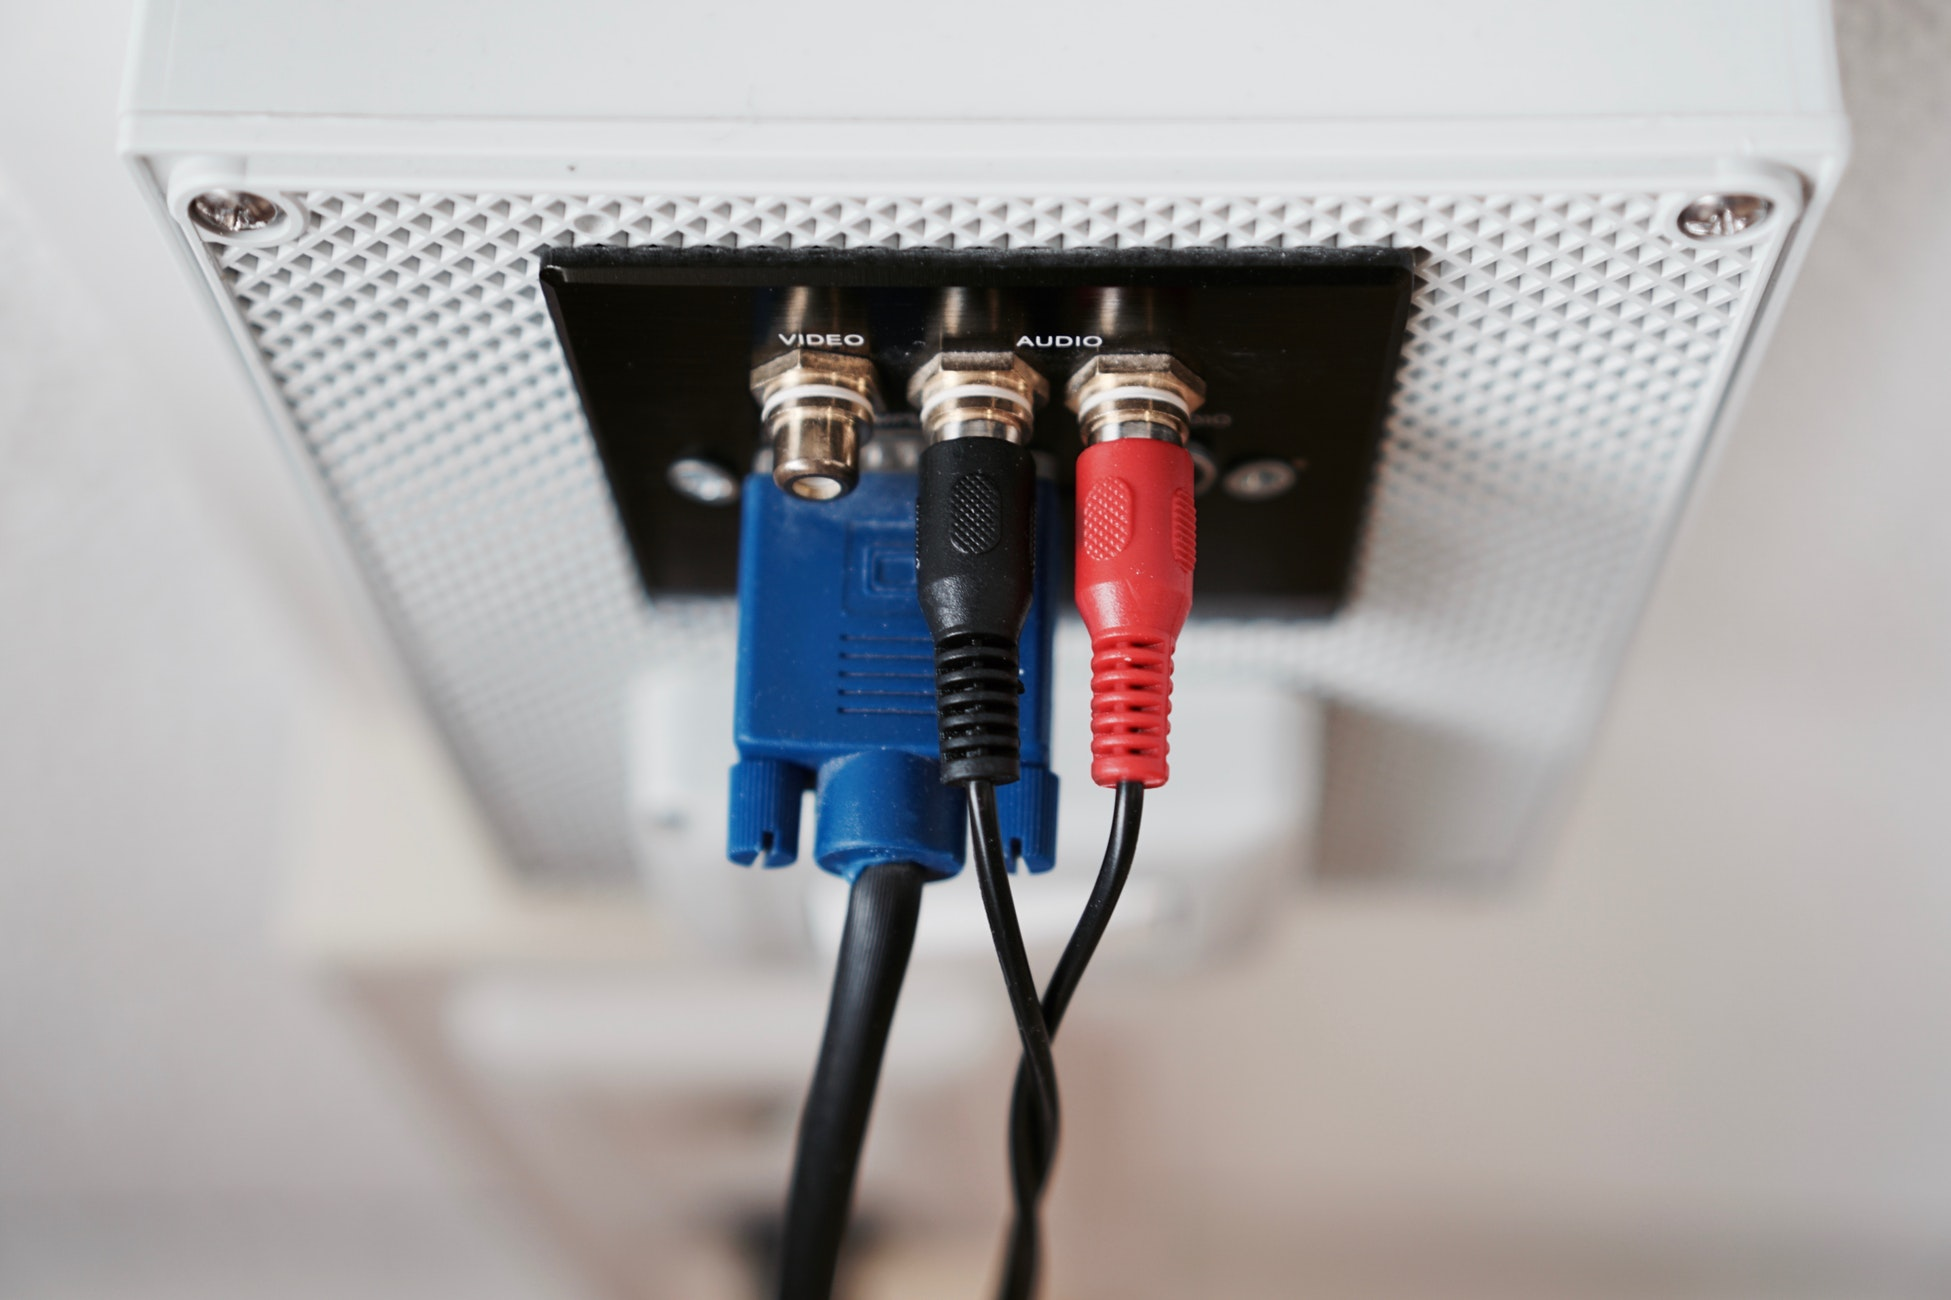
\includegraphics[width=0.60\textwidth]{images/project_charter_photo}
\end{figure}
\vspace{0.5 in}
{\centering \huge \color{accentcolor} \sc \textbf{\teamname \\ \productname} \par}
\vspace{0.5 in}
{\centering \large \sc \textbf{\authors} \par}
\newpage


%\vspace{1 in}
%\centerline{January 13th, 2012}
%\newpage

%%% Revision History
\begin{versionhistory}
  	\vhEntry{0.0.1}{11.20.2018}{AS}{Document creation}
  	\vhEntry{1.1.0}{11.30.2018}{AS}{Introduction}
  	\vhEntry{1.6.0}{11.30.2018}{UO}{Music Amplification/Speaker Subsystems}
  	\vhEntry{1.6.1}{11.30.2018}{UO}{Audio Amplifier}
  	\vhEntry{1.2.0}{11.31.2018}{JS}{System Overview}
  	\vhEntry{1.2.1}{11.31.2018}{JS}{Music Player Description}
  	\vhEntry{1.2.2}{11.31.2018}{JS}{Music Filter Description}
  	\vhEntry{1.2.3}{11.31.2018}{JS}{Audio Amplification/Speakers Description}
  	\vhEntry{1.3.0}{11.31.2018}{JS}{Subsystem Definitions and Data Flow}
  	\vhEntry{1.4.2}{12.01.2018}{CT}{Raspberry Pi}
  	\vhEntry{1.6.2}{12.01.2018}{CT}{Speakers}
  	\vhEntry{1.4.0}{12.02.2018}{AS}{Music Player Subsystems}
  	\vhEntry{1.4.1}{12.02.2018}{AS}{Website}
  	\vhEntry{1.5.0}{12.02.2018}{SO}{Music Filter Subsystems}
  	\vhEntry{1.5.1}{12.02.2018}{SO}{Pre-Amp}
  	\vhEntry{1.5.2}{12.02.2018}{SO}{Audio Filters}
  	\vhEntry{0.0.2}{12.02.2018}{SO|UO|JS|AS|CT}{complete draft}
  	\vhEntry{2.0.0}{12.04.2018}{SO|UO|JS|AS|CT}{official release}
\end{versionhistory}
\newpage

%%% Table of contents
\setcounter{tocdepth}{2}
\tableofcontents
\newpage

%%% List of figures and tables (optional)
\listoffigures
\listoftables
\newpage

%%% Document sections
\section{Introduction}
The sound backpack will take in a song, filter the low, mid, and high frequencies, then pass those frequencies to different shakers inside the backpack. The shakers will emit a vibration in time with the music so users can feel the beat.

The sound backpack will be available for purchase by the general public, but it will be designed and targeted for customers with hearing disabilities. Age restrictions may apply after evaluating the complexity of the final product.

The backpack will have a simple 2-way switch to serve as the powering on system, as well as a Volume/Intensity Knob and potentiometer for adjusting intensity of the music.
\newpage
\section{System Overview}
Product will be a vest, custom made, from a light weight material. The vest will be one size fits all, with adjustable straps for comfort. Several haptic motor controllers will be strategically sewn into the chest of the vest, along with a micro-controller and button control panel. The motors will vibrate within the vest according to the tempo of music played by the user. The music will be supplied and transmitted to the vest through Spotify API calls. The user will be able to log into the vest’s web based application to select music to play through the vest. The music will play in audio through the device accessing the web app, as well as vibrate through the vest. Profile settings and advanced vest settings can be set in the vest’s web application. The button controls on the vest will allow the customer to make local changes to the function of the vest, like vibration intensity. The vest will receive sound waves and instructions for the motors from a raspberry pi micro controller. The micro-controller will filter through sound waves and send instruction to the motors.
\newpage
\section{Subsystem Definitions \& Data Flow}
This section breaks down your layer abstraction to another level of detail. Here you grapically represent the logical subsytems that compose each layer and show the interactions/interfaces between those subsystems. A subsystem can be thought of as a programming unit that implements one of the major functions of the layer. It, therefore, has data elements that serve as source/sinks for other subsystems. The logical data elements that flow between subsystems need to be explicitly defined at this point, beginning with a data flow-like diagram based on the block diagram.

\begin{figure}[h!]
	\centering
 	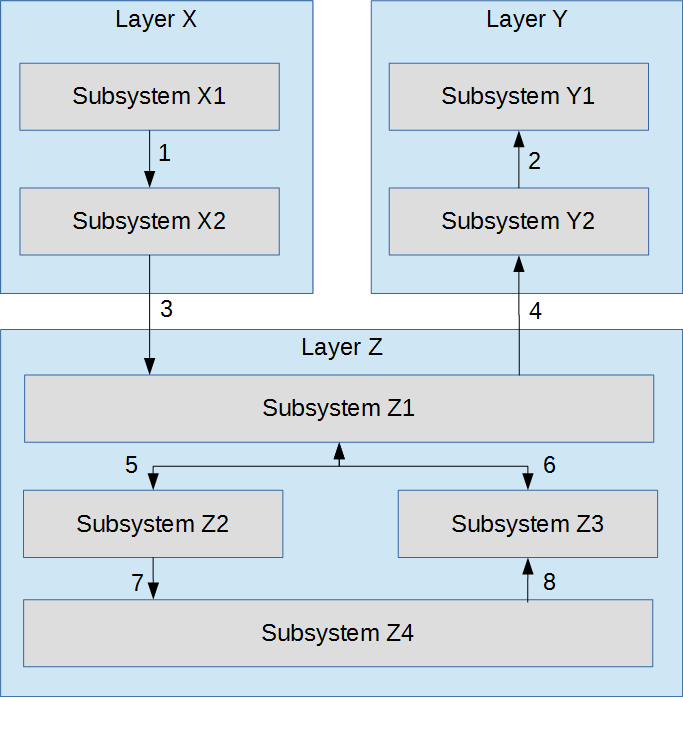
\includegraphics[width=\textwidth]{images/data_flow}
 \caption{A simple data flow diagram}
\end{figure}

\newpage
\section{Music Player Subsystems}
The first layer of the backpack is the music player layer. This layer is responsible for connecting the music player to the backpack and the backpack website. The different subsystems within this layer are the music player, the website, and the Raspberry Pi. The music player system is contingent upon whatever device/player the user prefers. This is a black-box system that will not be designed by the Sound Squad team.

\subsection{Website}
The website will serve as a means of product information/instructions, possible play list creation and management, and point of sale for purchase of other Sound Squad items. The website will communicate with the music player using API calls, and communicate with the backpack through a programmed connection with the backpack's Raspberry Pi. The website will have a database subsystem for user authentication and saving user settings and playlists.

\begin{figure}[h!]
	\centering
 	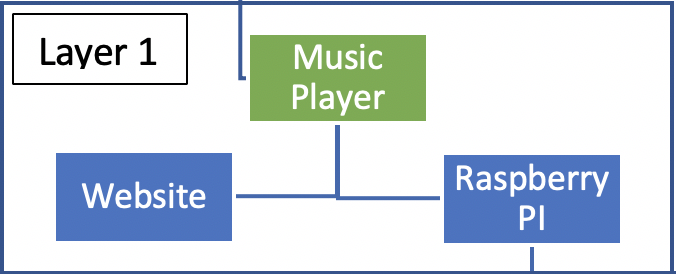
\includegraphics[width=0.60\textwidth]{images/subsystem1}
 \caption{Music player subsystem - website}
\end{figure}

\subsubsection{Assumptions}
Sound squad has made the assumption that APIs exist for all required functionality and interface between the website and the music player. Sound squad also made the assumption that users will have Wifi for the connection of the website changes to the Raspberry Pi.

\subsubsection{Responsibilities}
The website will be responsible for allowing the user to login to the Sound Squad site and connect to the music player site, make purchases of new products, create playlists and select songs to play, and finally to make advanced settings changes.

\subsubsection{Subsystem Interfaces}
The website will make an API call out to the music player and receive a rest endpoint containing the request/data. The website will connect to a Raspberry Pi via WiFi.

\begin {table}[H]
\caption {Website interfaces} 
\begin{center}
    \begin{tabular}{ | p{1cm} | p{6cm} | p{3cm} | p{3cm} |}
    \hline
    ID & Description & Inputs & Outputs \\ \hline
    \#1 & Connection to the music player & \pbox{3cm}{API call} & \pbox{3cm}{API endpoint}  \\ \hline
    \#2 & Connection to the Raspberry Pi & \pbox{3cm}{NA} & \pbox{3cm}{Music signal}  \\ \hline
    \end{tabular}
\end{center}
\end{table}

\subsection{Raspberry Pi}
The Raspberry Pi will act as the medium between the music player layer and the music filter layer. It receives and passes on any audio signals it receives. It also receives and passes on any relevant instructions from the website. The Raspberry Pi will be maintaining a WiFi connection with the website, while also receiving and sending audio signals.

\begin{figure}[h!]
	\centering
 	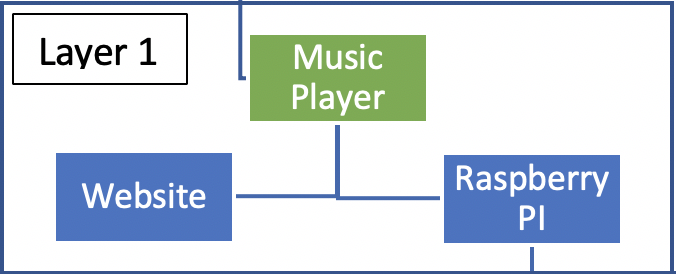
\includegraphics[width=0.60\textwidth]{images/subsystem1}
 \caption{Music player subsystem - Raspberry Pi}
\end{figure}

\subsubsection{Assumptions}
We assume that a Raspberry Pi that meets our specifications is readily available. We also assume that the Raspberry Pi will be capable of maintaining a WiFi connection, and that it will be able to efficiently receive and pass on the music signals. Finally, we assume that, if any peripheral attachments for the Raspberry Pi are needed for our system, they will also be readily available.

\subsubsection{Responsibilities}
The Raspberry Pi is responsible for maintaining a connection to the website and the music player. It needs to maintain a Wifi connection with the website. It is also the responsibility of the Raspberry Pi to forward the music signals to the pre-amp. It must also take in and pass on any user-given changes in audio settings.

\subsubsection{Subsystem Interfaces}

\begin {table}[H]
\caption {Raspberry Pi interfaces} 
\begin{center}
    \begin{tabular}{ | p{1cm} | p{6cm} | p{3cm} | p{3cm} |}
    \hline
    ID & Description & Inputs & Outputs \\ \hline
    \#1 & WiFi Connection to Website & \pbox{3cm}{ Changes on website } & \pbox{3cm}{ Raspberry Pi sends changes to appropriate system }  \\ \hline
    \#2 & Connection to the music player & \pbox{3cm}{ Music/audio signals } & \pbox{3cm}{ Music/audio signals sent to pre-amp }  \\ \hline
    \end{tabular}
\end{center}
\end{table}




\newpage
\section{Music Filter Subsystems}
In this section, the layer is described in some detail in terms of its specific subsystems. Describe each of the layers and its subsystems in a separate chapter/major subsection of this document. The content of each subsystem description should be similar. Include in this section any special considerations and/or trade-offs considered for the approach you have chosen.

\subsection{Pre-Amp}
This section should be a general description of a particular subsystem for the given layer. For most subsystems, an extract of the architectural block diagram with data flows is useful. This should consist of the subsystem being described and those subsystems with which it communicates.

\begin{figure}[h!]
	\centering
 	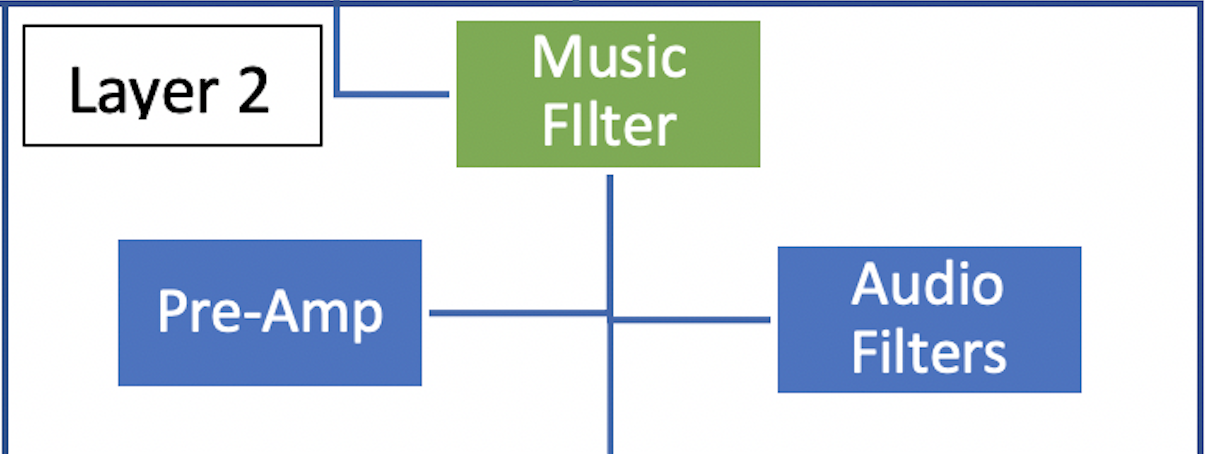
\includegraphics[width=0.60\textwidth]{images/subsystem2}
 \caption{Example subsystem description diagram}
\end{figure}

\subsubsection{Assumptions}
Any assumptions made in the definition of the subsystem should be listed and described. Pay particular attention to assumptions concerning interfaces and interactions with other layers.

\subsubsection{Responsibilities}
Each of the responsibilities/features/functions/services of the subsystem as identified in the architectural summary must be expanded to more detailed responsibilities. These responsibilities form the basis for the identification of the finer-grained responsibilities of the layer's internal subsystems. Clearly describe what each subsystem does.

\subsubsection{Subsystem Interfaces}
Each of the inputs and outputs for the subsystem are defined here. Create a table with an entry for each labelled interface that connects to this subsystem. For each entry, describe any incoming and outgoing data elements will pass through this interface.

\begin {table}[H]
\caption {Subsystem interfaces} 
\begin{center}
    \begin{tabular}{ | p{1cm} | p{6cm} | p{3cm} | p{3cm} |}
    \hline
    ID & Description & Inputs & Outputs \\ \hline
    \#xx & Description of the interface/bus & \pbox{3cm}{input 1 \\ input 2} & \pbox{3cm}{output 1}  \\ \hline
    \#xx & Description of the interface/bus & \pbox{3cm}{N/A} & \pbox{3cm}{output 1}  \\ \hline
    \end{tabular}
\end{center}
\end{table}

\subsection{Audio Filters}
This section should be a general description of a particular subsystem for the given layer. For most subsystems, an extract of the architectural block diagram with data flows is useful. This should consist of the subsystem being described and those subsystems with which it communicates.

\begin{figure}[h!]
	\centering
 	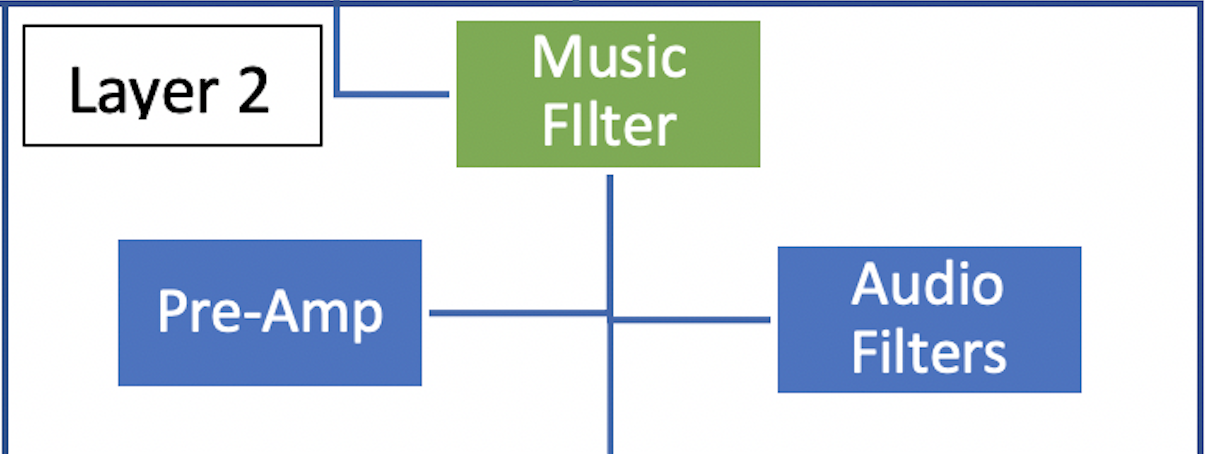
\includegraphics[width=0.60\textwidth]{images/subsystem2}
 \caption{Example subsystem description diagram}
\end{figure}

\subsubsection{Assumptions}
Any assumptions made in the definition of the subsystem should be listed and described. Pay particular attention to assumptions concerning interfaces and interactions with other layers.

\subsubsection{Responsibilities}
Each of the responsibilities/features/functions/services of the subsystem as identified in the architectural summary must be expanded to more detailed responsibilities. These responsibilities form the basis for the identification of the finer-grained responsibilities of the layer's internal subsystems. Clearly describe what each subsystem does.

\subsubsection{Subsystem Interfaces}
Each of the inputs and outputs for the subsystem are defined here. Create a table with an entry for each labelled interface that connects to this subsystem. For each entry, describe any incoming and outgoing data elements will pass through this interface.

\begin {table}[H]
\caption {Subsystem interfaces} 
\begin{center}
    \begin{tabular}{ | p{1cm} | p{6cm} | p{3cm} | p{3cm} |}
    \hline
    ID & Description & Inputs & Outputs \\ \hline
    \#xx & Description of the interface/bus & \pbox{3cm}{input 1 \\ input 2} & \pbox{3cm}{output 1}  \\ \hline
    \#xx & Description of the interface/bus & \pbox{3cm}{N/A} & \pbox{3cm}{output 1}  \\ \hline
    \end{tabular}
\end{center}
\end{table}


\newpage
\section{Music Amplification/Speaker Subsystems}
In this section, the layer is described in some detail in terms of its specific subsystems. Describe each of the layers and its subsystems in a separate chapter/major subsection of this document. The content of each subsystem description should be similar. Include in this section any special considerations and/or trade-offs considered for the approach you have chosen.

\subsection{Audio Amplifier}
This section should be a general description of a particular subsystem for the given layer. For most subsystems, an extract of the architectural block diagram with data flows is useful. This should consist of the subsystem being described and those subsystems with which it communicates.

\begin{figure}[h!]
	\centering
 	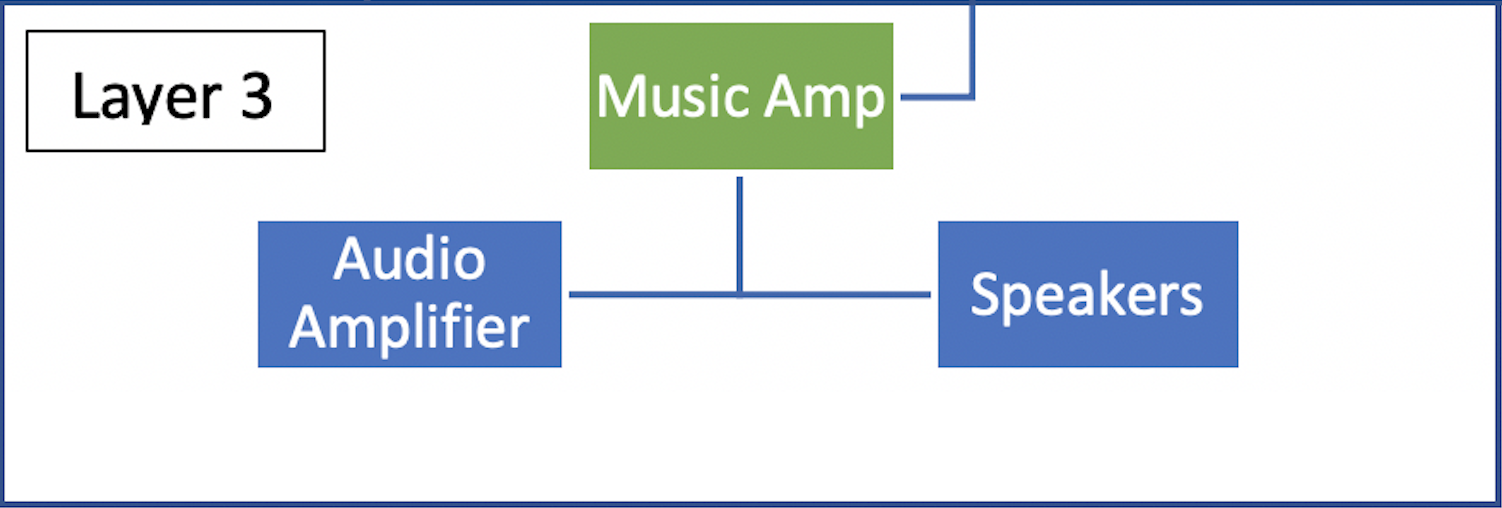
\includegraphics[width=0.60\textwidth]{images/subsystem3}
 \caption{Example subsystem description diagram}
\end{figure}

\subsubsection{Assumptions}
Any assumptions made in the definition of the subsystem should be listed and described. Pay particular attention to assumptions concerning interfaces and interactions with other layers.

\subsubsection{Responsibilities}
Each of the responsibilities/features/functions/services of the subsystem as identified in the architectural summary must be expanded to more detailed responsibilities. These responsibilities form the basis for the identification of the finer-grained responsibilities of the layer's internal subsystems. Clearly describe what each subsystem does.

\subsubsection{Subsystem Interfaces}
Each of the inputs and outputs for the subsystem are defined here. Create a table with an entry for each labelled interface that connects to this subsystem. For each entry, describe any incoming and outgoing data elements will pass through this interface.

\begin {table}[H]
\caption {Subsystem interfaces} 
\begin{center}
    \begin{tabular}{ | p{1cm} | p{6cm} | p{3cm} | p{3cm} |}
    \hline
    ID & Description & Inputs & Outputs \\ \hline
    \#xx & Description of the interface/bus & \pbox{3cm}{input 1 \\ input 2} & \pbox{3cm}{output 1}  \\ \hline
    \#xx & Description of the interface/bus & \pbox{3cm}{N/A} & \pbox{3cm}{output 1}  \\ \hline
    \end{tabular}
\end{center}
\end{table}

\subsection{Speakers}
The speakers are one of the last, most straightforward systems in the vest. There will be three sets of speakers for different frequencies: lows, mids, and highs. These will act as the shakers for the vest. The speakers will also act simply as a medium for output, and will do no heavy-duty signal processing of their own. It will be connected to the music amp and the audio amplifier. The speakers are a black-box system that will not be designed by the team.

\begin{figure}[h!]
	\centering
 	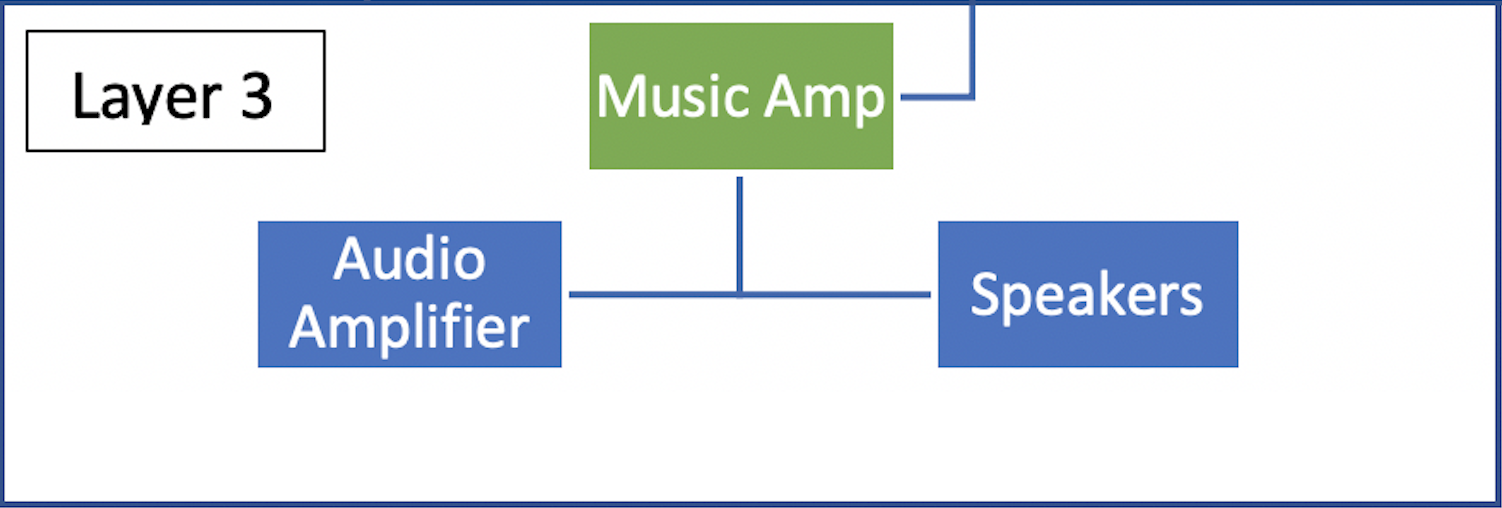
\includegraphics[width=0.60\textwidth]{images/subsystem3}
 \caption{Example subsystem description diagram}
\end{figure}

\subsubsection{Assumptions}
It is assumed that there will be speakers available that will fit our specifications and that will be able to comfortably and safely fit in the vest. We also assume that there are speakers powerful enough to emit vibrations that can be felt through the vest we will use.

\subsubsection{Responsibilities}
The speakers have few responsibilities, in terms of custom functionality. They are simply meant to be the medium through which the user will feel the music/vibrations.

\subsubsection{Subsystem Interfaces}

\begin {table}[H]
\caption {Subsystem interfaces} 
\begin{center}
    \begin{tabular}{ | p{1cm} | p{6cm} | p{3cm} | p{3cm} |}
    \hline
    ID & Description & Inputs & Outputs \\ \hline
    \#1 & Connection to audio amplifier & \pbox{3cm}{ Audio amplification settings } & \pbox{3cm}{ Change in audio/vibration characteristics in vest }  \\ \hline
    \#2 & Connection to music amplifier & \pbox{3cm}{ NA } & \pbox{3cm}{ Speakers receive amplified audio/music signals ready for output }  \\ \hline
    \end{tabular}
\end{center}
\end{table}


\newpage

%%% References
\bibliographystyle{plain}
\bibliographystyle{reference/IEEEtran_custom}
\bibliography{reference/refs}{}

\end{document}